\documentclass[11pt]{article}
\usepackage[letterpaper,margin=1in]{geometry}
\usepackage{mytex}

\usepackage[dvipsnames]{xcolor}
\usepackage[colorlinks=true, citecolor=MidnightBlue, linkcolor=MidnightBlue]{hyperref} % hyperlinks


\usepackage{bookmark}



\usepackage{newtxtext, kotex}
\usepackage[all,cmtip]{xy}

\usepackage{tikz}
\usepackage{tikz-cd}
\usetikzlibrary{calc,positioning}
\usetikzlibrary{arrows.meta,calc,positioning,fit,backgrounds}

\usepackage{pgfplots}
\usepackage{caption}

\usepackage{fancyhdr}
%\fancyhf{} % sets both header and footer to nothing
\renewcommand{\headrulewidth}{0pt}



\usepackage[textwidth=.85in,textsize=scriptsize,colorinlistoftodos]{todonotes} % todo 노트

\pagestyle{fancy}
\lhead{Myungsin Cho}
\chead{}
\rhead{}
%\rfoot{\date}



%Bibliography line spacing
% ADD THE FOLLOWING COUPLE LINES INTO YOUR PREAMBLE
\let\OLDthebibliography\thebibliography
\renewcommand\thebibliography[1]{
  \OLDthebibliography{#1}
  \setlength{\parskip}{0pt}
  \setlength{\itemsep}{0pt plus 0.3ex}
}

% section 폰트 바꿔주는거
\usepackage{titlesec}
\titleformat{\section}{\normalfont\large\center}{\thesection}{.5em}{}
\titleformat{\subsection}[runin]{\normalfont\bfseries}{\thesubsection}{.5em}{}

\newcommand{\yourname}{Myungsin Cho}

\newcommand\quelle[1]{{%
      \unskip\nobreak\hfil\penalty50
      \hskip2em\hbox{}\nobreak\hfil #1%
      \parfillskip=0pt \finalhyphendemerits=0 \par}}
      

\usepackage{amsmath,amsfonts,amssymb,mathrsfs}
\usepackage{amsthm,thmtools}
\newtheorem{theorem}{Theorem}
\newtheorem*{wip}{Work in progress}
\newtheorem{proposition}{Proposition}
\newtheorem{lemma}{Lemma}
\newtheorem{corollary}[theorem]{Corollary}
\newtheorem*{goal}{Goal}
\newtheorem*{conjecture}{Conjecture}

\let\overto\xrightarrow

\newcommand{\KR}{\operatorname{KR}}
\newcommand{\K}{\operatorname{K}}
\newcommand{\LK}{{L_{K(1)}}}
\newcommand{\THH}{\operatorname{THH}}
\newcommand{\GW}{\operatorname{GW}}
\newcommand{\TC}{\operatorname{TC}}
\newcommand{\U}{\operatorname{U}}


\author{Myungsin Cho}
\date{}
\begin{document}
\begin{center}\LARGE{Research Statement}\end{center}\vspace{.5em}
My research is in stable homotopy theory, with connections to arithmetic and equivariant algebra.
I study how mathematical invariants are related by duality and how global information can be recovered from local data through descent.
My central goal is to understand these phenomena in Real algebraic $K$-theory, where algebraic objects carry an order-two symmetry.
My work develops this program through arithmetic duality, computational methods, and the algebra of objects with symmetry.

\section*{Arithmetic duality and Real algebraic $K$-theory}
Algebraic $K$-theory studies rings through invariants built from their projective modules.
For number fields, it connects topology to arithmetic by comparing global objects with their completions at individual primes.
Classical Tate--Poitou duality describes such relationships through cohomology.
Descent connects this cohomological information to a localized form of $K$-theory, raising the question of whether the arithmetic duality also holds for the underlying spectra.

My dissertation establishes $K$-theoretic Tate--Poitou duality at the prime $2$, completing the global duality previously proved at odd primes by Blumberg and Mandell.
The remaining case required accounting for the additional behavior of real embeddings.
The theorem shows that the comparison between global and local $K$-theory has a duality symmetry: global $K$-theory is dual to the term measuring the difference between global and local data, while local $K$-theory is self-dual.
Here the appropriate homotopical dual is the $2$-adic Anderson dual.
The result establishes a duality of spectra, including the structure connecting their homotopy groups.

This duality also has an application to the $K$-theory of the sphere spectrum, a fundamental object in stable homotopy theory.
The cyclotomic trace approximates this difficult invariant by a more computable one.
At the prime $2$ and in nonnegative degrees, my theorem identifies the information missed by this approximation in terms of the arithmetic $K$-theory of the integers.

Real algebraic $K$-theory combines ordinary $K$-theory with Grothendieck--Witt theory ($\GW$), which studies modules equipped with nondegenerate bilinear forms.
With Lucy Yang, I establish a compatible duality over $2$-adic local fields for the sequence connecting $\GW$, $K$-theory, and its comparison theory $\U$.
Our ongoing work seeks a global duality encompassing all three theories.
In the diagram below, each row compares global and local data, while each column connects the three theories.
The red row and blue column show the dualities already obtained.
We expect the full diagram to be self-dual under a half-turn rotation.
\begin{center}
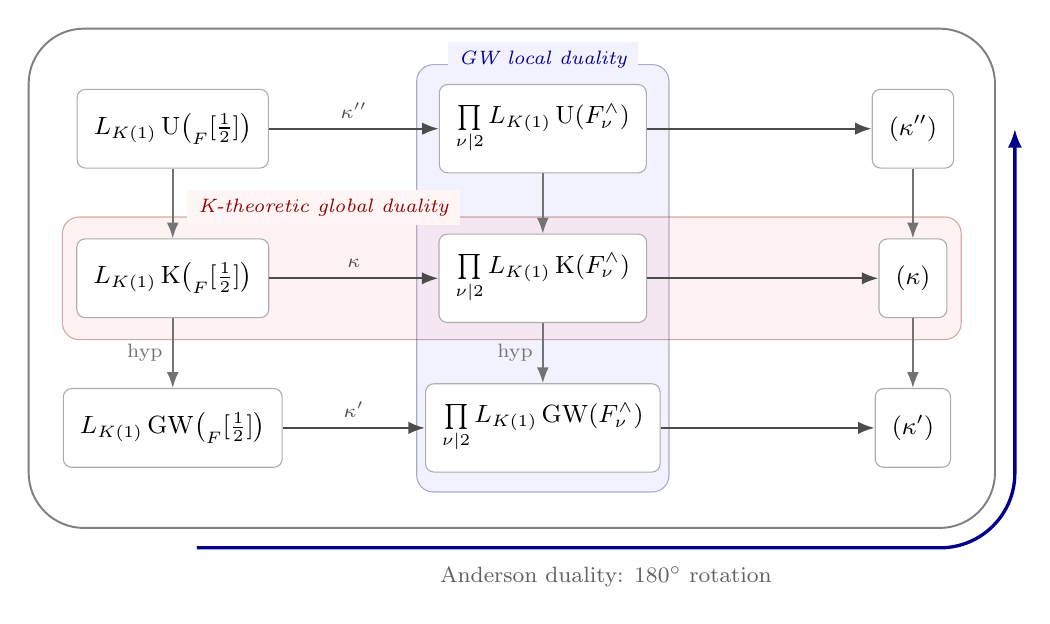
\begin{tikzpicture}[
  >=Latex,
  x=1cm,
  y=1cm,
  term/.style={
    draw=black!32,
    fill=white,
    rounded corners=3pt,
    inner xsep=6pt,
    inner ysep=7pt,
    align=center,
    font=\small,
    minimum height=1.00cm
  },
  seq/.style={-{Latex[length=2.1mm]},thick,black!70},
  vert/.style={-{Latex[length=2mm]},semithick,black!55},
  rotation/.style={{Latex[length=2.4mm]}-,very thick,blue!55!black}
]

% U-row
\node[term] (Ug) at (-4.7,1.9)
  {$L_{K(1)}\operatorname{U}\bigl(\calO_F[\tfrac12]\bigr)$};
\node[term] (Ul) at (0,1.9)
  {$\prod\limits_{\nu\mid2}L_{K(1)}\operatorname{U}(F_\nu^\wedge)$};
\node[term] (Uc) at (4.7,1.9)
  {$\Cof(\kappa'')$};

% K-row
\node[term] (Kg) at (-4.7,0)
  {$L_{K(1)}\K\bigl(\calO_F[\tfrac12]\bigr)$};
\node[term] (Kl) at (0,0)
  {$\prod\limits_{\nu\mid2}L_{K(1)}\K(F_\nu^\wedge)$};
\node[term] (Kc) at (4.7,0)
  {$\Cof(\kappa)$};

% GW-row
\node[term] (GWg) at (-4.7,-1.9)
  {$L_{K(1)}\GW\bigl(\calO_F[\tfrac12]\bigr)$};
\node[term] (GWl) at (0,-1.9)
  {$\prod\limits_{\nu\mid2}L_{K(1)}\GW(F_\nu^\wedge)$};
\node[term] (GWc) at (4.7,-1.9)
  {$\Cof(\kappa')$};

% Horizontal cofiber sequences
\draw[seq] (Ug) -- node[above,font=\scriptsize] {$\kappa''$} (Ul);
\draw[seq] (Ul) -- (Uc);
\draw[seq] (Kg) -- node[above,font=\scriptsize] {$\kappa$} (Kl);
\draw[seq] (Kl) -- (Kc);
\draw[seq] (GWg) -- node[above,font=\scriptsize] {$\kappa'$} (GWl);
\draw[seq] (GWl) -- (GWc);

% Vertical cofiber sequences
\draw[vert] (Ug) -- (Kg);
\draw[vert] (Kg) -- node[left,font=\scriptsize] {$\operatorname{hyp}$} (GWg);
\draw[vert] (Ul) -- (Kl);
\draw[vert] (Kl) -- node[left,font=\scriptsize] {$\operatorname{hyp}$} (GWl);
\draw[vert] (Uc) -- (Kc);
\draw[vert] (Kc) -- (GWc);


% The labels make the two colors self-explanatory.
\node[
  anchor=west,
  font=\scriptsize\itshape,
  text=red!58!black,
  fill=red!4,
  inner xsep=4pt
] at (-4.52,0.9)
  {K-theoretic global duality};

\node[
  anchor=center,
  font=\scriptsize\itshape,
  text=blue!58!black,
  fill=blue!5,
  inner xsep=4pt
] at (0,2.78)
  {GW local duality};


% Backgrounds: the earlier theorem is a horizontal slice of the larger diagram.
\begin{scope}[on background layer]
  \node[
    fit=(Ul)(Kl)(GWl),
    rounded corners=6pt,
    fill=blue!38,
    fill opacity=.13,
    draw=blue!48!black,
    draw opacity=.32,
    inner xsep=3pt,
    inner ysep=7pt
  ] (localslice) {};
  
  \node[
    fit=(Kg)(Kl)(Kc),
    rounded corners=6pt,
    fill=red!38,
    fill opacity=.13,
    draw=red!48!black,
    draw opacity=.32,
    inner xsep=5pt,
    inner ysep=6pt
  ] (kslice) {};

  \node[
    fit=(Ug)(Ul)(Uc)(GWg)(GWl)(GWc)(kslice),
    rounded corners=20pt,
  draw=black!50,
    line width=.7pt,
    inner xsep=12pt,
    inner ysep=20pt
  ] (whole) {};
\end{scope}

\def\dualitygap{0.24}

\draw[
  rotation,
  rounded corners=27pt
]
  ($(whole.east |- Uc.east)+(\dualitygap,0)$)
  -- ($(whole.south east)+(\dualitygap,-\dualitygap)$)
  --
  node[
    midway,
    below=3pt,
    inner xsep=0pt,
    font=\footnotesize,
    text=black!62
  ] {Anderson duality: $180^\circ$ rotation}
  ($(whole.south)+(-4,-\dualitygap)$);
\end{tikzpicture}
\end{center}

\newpage
\section*{Toward equivariant duality and descent}
I conjecture that these arithmetic dualities arise from a single duality in Real algebraic $K$-theory.
Forgetting the symmetry should recover my dissertation theorem, while the equivariant structure should explain the compatible dualities of the three theories in the diagram.
In ordinary $K$-theory, descent explains how arithmetic duality passes from cohomology to spectra.
A corresponding equivariant cohomology theory for Real algebraic $K$-theory is not yet available.
I therefore approach the problem from the other direction, using the expected duality to guide the construction of a Real descent theory.

\section*{Real trace methods}
Trace methods make algebraic $K$-theory more accessible by replacing it with invariants that are easier to compute.
In joint work with Gerhardt, Keenan, Moreno, and Quigley, I develop Real versions of these methods that also account for symmetry.
We construct a multiplicative spectral sequence, a tool that organizes a computation into successive stages, and carry out explicit calculations for Real bordism theories.
The construction respects the additional algebraic operations arising from equivariance and extends the methods of Bruner and Rognes to the Real setting.
My next goal is a Real Segal conjecture for Real complex bordism and Real Brown--Peterson theory.
This would deepen our understanding of these computational approximations and provide input for studying Real algebraic $K$-theory beyond number fields.

\section*{Equivariant algebra}
Symmetry introduces additional forms of addition and multiplication, called transfers and norms.
With Chan, Mehrle, Sanchez Ocal, Osorno, Szczesny, and Verdugo, I study when combinatorial descriptions of these operations can be realized by operads governing their interaction.
We prove realization when all additive transfers are available, establish further cases, and conjecture realization for every compatible pair of transfer systems.

With Noah Wisdom, I study how representation gradings organize the homotopy groups of equivariant spectra.
For the order-two group, within the class of gradings modeled on stable homotopy groups, we show that the extra symmetries of representation degrees are already determined by the Mackey functor structure.


\bibliography{RS_bib}
\bibliographystyle{alphaurl}

\end{document}